\section{内层响应法}
\label{sec:minimax-inner-response}

最直接的求解办法是照着决策顺序来：固定当前的$\bm{x}$，先求最坏响应，再用值函数的信息更新$\bm{x}$。外层用什么算法，前面各章已经讲过，本节只回答两个新问题：内层要解到什么程度，内层的误差怎样传到外层。

图~\ref{fig:minimax-response-flow}是整个方法的结构。

\begin{BookInlineFigure}
 \centering
 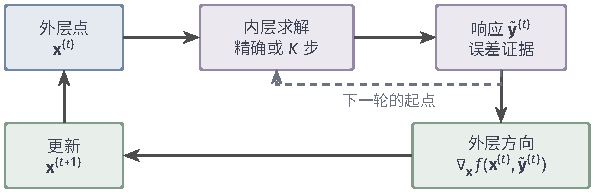
\includegraphics[width=100.7mm]{figures/05-optimization/07-multiple-criteria-and-nested-optimization/tikz/minimax-response-flow/figure.pdf}
 \caption{内层响应法的一轮。紫框是内层计算，绿框是外层计算。内层的输出除了响应，还应带有它的误差证据。虚线表示本轮响应作为下一轮内层的起点。}
 \label{fig:minimax-response-flow}
\end{BookInlineFigure}

\subsection{精确响应}
\label{sec:minimax-exact-response}

\paragraph{主要思想}
设内层最优响应唯一且$\phi$可微。定理~\ref{thm:minimax-danskin}说，算梯度时可以把响应当作常数，所以外层的梯度步就是
\begin{equation}
 \bm{x}^{(t+1)}=P_{\bm{X}}\Bigl(\bm{x}^{(t)}-\alpha\nabla_{\bm{x}}f\bigl(\bm{x}^{(t)},\bm{y}^\star(\bm{x}^{(t)})\bigr)\Bigr),
 \label{eq:minimax-exact-step}
\end{equation}
其中$\bm{X}$是闭凸集，$P_{\bm{X}}$是第~\ref{chap:feasible-iterations}章的欧氏投影，$\bm{X}=\mathbb{R}^n$时投影是恒等映射。这就是对$\phi$做投影梯度法，收敛性由$\phi$的光滑常数和凸性决定，不需要新的理论。

\paragraph{计算过程}
用式~\eqref{eq:minimax-running-phi}的函数演示，$f=-\frac12x^2+2xy-\frac12y^2$，$X=Y=\mathbb{R}$。

\needspace{6\baselineskip}
\paragraph{变量}
\begin{itemize}
 \item $x^{(t)}$：外层变量；
 \item $y^{(t)}$：内层在$x^{(t)}$处的精确响应；
 \item $g^{(t)}$：外层偏导数；
 \item $\alpha>0$：外层步长。
\end{itemize}

\paragraph{初始化}
取$x^{(0)}$。例中$x^{(0)}=1$，步长$\alpha=\frac16$，当$\lvert g^{(t)}\rvert\leq0.4$时停止。

\needspace{6\baselineskip}
\paragraph{每轮更新}
\begin{enumerate}
 \item 解内层，得$y^{(t)}=y^\star(x^{(t)})$。例中$y^\star(x)=2x$，第一轮
 \[
  y^{(0)}=2.
 \]
 \item 计算外层偏导数$g^{(t)}=\partial_xf(x^{(t)},y^{(t)})$。例中$\partial_xf=-x+2y$，第一轮
 \[
  g^{(0)}=-1+4=3.
 \]
 \item 由式~\eqref{eq:minimax-exact-step}更新。例中第一轮
 \[
  x^{(1)}=1-\frac16\cdot3=\frac12.
 \]
\end{enumerate}

第二轮$y^{(1)}=1$，$g^{(1)}=\frac32$，$x^{(2)}=\frac14$。第三轮$y^{(2)}=\frac12$，$g^{(2)}=\frac34$，$x^{(3)}=\frac18$。第四轮$y^{(3)}=\frac14$，$g^{(3)}=\frac38\leq0.4$，停止。

最终得到$x^{(3)}=\frac18$，最坏值$\phi(\frac18)=\frac{3}{128}$。例中$g^{(t)}=\phi'(x^{(t)})=3x^{(t)}$，与式~\eqref{eq:minimax-running-phi}的导数相同，这正是定理~\ref{thm:minimax-danskin}的内容。

\paragraph{响应切换时改用非光滑方法}
$\phi$有折角时，式~\eqref{eq:minimax-exact-step}里的偏梯度只是一个次梯度，而次梯度不随接近解而变小。设$f=(x-y)^2$，$Y=[-1,1]$，$x^{(0)}=0.8$，固定步长$\alpha=0.2$。

$x>0$时最坏响应是$y=-1$，偏导数是$2(x+1)$；$x<0$时最坏响应是$y=1$，偏导数是$2(x-1)$。前三步是
\[
 \begin{aligned}
 x^{(1)}&=0.8-0.2\cdot3.6=0.08,\\
 x^{(2)}&=0.08-0.2\cdot2.16=-0.352,\\
 x^{(3)}&=-0.352+0.2\cdot2.704=0.1888.
 \end{aligned}
\]

迭代很快进入一个周期为$2$的循环。在循环上，$x>0$时映射是$x\mapsto0.6x-0.4$，$x<0$时映射是$x\mapsto0.6x+0.4$，解$a\mapsto-a\mapsto a$得到$a=\frac14$。迭代在$\pm\frac14$之间来回跳，目标差停在$(\frac54)^2-1=0.5625$，见图~\ref{fig:minimax-subgradient-worst}中的黄线。

\begin{BookInlineFigure}
 \centering
 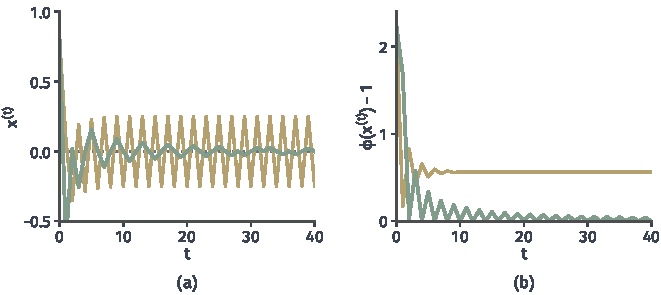
\includegraphics[width=112mm]{figures/05-optimization/07-multiple-criteria-and-nested-optimization/matplotlib/minimax-subgradient-worst/figure.pdf}
 \caption{精确响应加次梯度步，$\phi(x)=(\lvert x\rvert+1)^2$，起点$0.8$。黄线是固定步长$0.2$，绿线是递减步长$0.4/(t+1)$。(a)迭代点：黄线进入$\pm\frac14$的循环，绿线逐渐收敛到最优解$0$。(b)目标差：黄线停在$0.5625$，绿线继续下降。}
 \label{fig:minimax-subgradient-worst}
\end{BookInlineFigure}

这是第~\ref{chap:nonsmooth-composite-optimization}章次梯度法的典型行为，$\phi$是凸函数时那里的结论可以直接使用：有界次梯度下，步长取固定值$R/(G_{\mathrm{b}}\sqrt{T})$时平均点的目标差不超过$RG_{\mathrm{b}}/\sqrt{T}$，其中$R$是起点到解的距离上界，$G_{\mathrm{b}}$是次梯度范数上界。要让误差继续减小，步长必须递减。

\paragraph{局部极大不能代替全局最坏响应}
定理~\ref{thm:minimax-danskin}要的是全局最优响应。内层不凹时，内层算法通常只能找到局部极大点。看下面的函数，$Y=[-2,2]$：
\begin{equation}
 f(x,y)=\frac12x^2+xy+y^2-\frac14y^4.
 \label{eq:minimax-nonconcave}
\end{equation}

固定$x=1$，令$\partial_yf=1+2y-y^3=0$。因式分解得到
\[
 (y+1)(y^2-y-1)=0,
\]
三个根是$y=-1$，$y=\frac{1+\sqrt5}{2}\approx1.618$，$y=\frac{1-\sqrt5}{2}\approx-0.618$。计算得到
\[
 f(1,-1)=0.25,\qquad f(1,1.618)\approx3.023,\qquad f(1,-0.618)\approx0.227.
\]
$y=-1$是局部极大，$y=1.618$是全局极大，$y=-0.618$是局部极小，见图~\ref{fig:minimax-local-response}(a)。

\begin{BookInlineFigure}
 \centering
 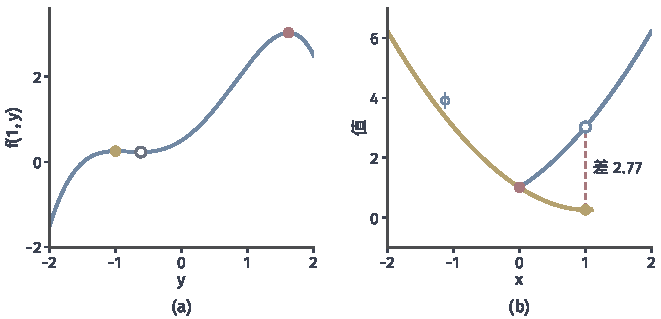
\includegraphics[width=112mm]{figures/05-optimization/07-multiple-criteria-and-nested-optimization/matplotlib/minimax-local-response/figure.pdf}
 \caption{内层不凹的例子，$f=\frac12x^2+xy+y^2-\frac14y^4$，$Y=[-2,2]$。(a)$x=1$时的内层函数：黄点是局部极大，红点是全局极大，空心点是局部极小。(b)蓝线是真实的$\phi$，红点是外层最优解；黄线是沿局部极大分支算得的值。$x=1$处两者相差$2.77$，局部分支到$x\approx1.089$处消失。}
 \label{fig:minimax-local-response}
\end{BookInlineFigure}

假设内层算法从$y<-0.618$的地方起步，它会收敛到$y=-1$。这一步的代价极大：报告的最坏值是$0.25$，真实值是$3.023$。更糟的是外层的方向，$\partial_xf=x+y$在这个响应处是
\[
 \partial_xf(1,-1)=0,
\]
看起来$x=1$已经驻定。而真实的导数是
\[
 \phi'(1)=1+1.618=2.618.
\]
图~\ref{fig:minimax-local-response}(b)中，黄线的局部分支一路下降，到$x=1$处还很低，蓝线的真实$\phi$却在升高。外层最优解其实是$x=0$，$\phi(0)=1$；局部分支报告的$0.25$甚至低于真正的最优值。

内层关于$\bm{y}$凹时，这个问题不存在，因为凹函数在凸集上的局部极大就是全局极大。否则，一个响应的“最优”只是相对于找到它的算法而言，后面报告结果时必须说明这一点。

\subsection{近似响应}
\label{sec:minimax-approx-response}

实际计算很少精确解内层，算到什么程度够用？先定义内层误差。

固定$\bm{x}$，对候选响应$\tilde{\bm{y}}\in\bm{Y}$，称
\begin{equation}
 \varepsilon=\phi(\bm{x})-f(\bm{x},\tilde{\bm{y}})\geq0
 \label{eq:minimax-inner-gap}
\end{equation}
为内层间隙。用它衡量比用$\bm{y}$的距离更合适，因为外层真正关心的是最坏值差多少。要把间隙转成外层梯度的误差，需要一座桥，这座桥就是强凹性：顶部越尖，间隙小就越能说明位置近，如同碗越陡，高度差小，水平距离就越小。

下面的条件贯穿本节。设$\bm{Y}$闭凸；$f$的梯度在$\bm{X}\times\bm{Y}$上$L$-Lipschitz；对每个$\bm{x}$，$f(\bm{x},\cdot)$在$\bm{Y}$上$\mu$强凹，$\mu>0$，记$\kappa=L/\mu$。

\begin{theorem}[内层间隙到外层梯度的传递]
\label{thm:minimax-inexact-gradient}
在上述条件下，内层响应唯一，记为$\bm{y}^\star(\bm{x})$。对任意$\tilde{\bm{y}}\in\bm{Y}$，
\begin{equation}
 \lVert\tilde{\bm{y}}-\bm{y}^\star(\bm{x})\rVert_2\leq\sqrt{\frac{2\varepsilon}{\mu}}.
 \label{eq:minimax-distance}
\end{equation}
进一步，
\begin{equation}
 \bigl\lVert\nabla_{\bm{x}}f(\bm{x},\tilde{\bm{y}})-\nabla_{\bm{x}}f(\bm{x},\bm{y}^\star(\bm{x}))\bigr\rVert_2\leq L\sqrt{\frac{2\varepsilon}{\mu}}.
 \label{eq:minimax-gradient-error}
\end{equation}
\end{theorem}

\begin{proof}
强凹函数在闭凸集上的最大点存在且唯一，记$\bm{y}^\star=\bm{y}^\star(\bm{x})$。最优性给出
\[
 \langle\nabla_{\bm{y}}f(\bm{x},\bm{y}^\star),\tilde{\bm{y}}-\bm{y}^\star\rangle\leq0.
\]
由$\mu$强凹的二次上界，
\[
 f(\bm{x},\tilde{\bm{y}})\leq f(\bm{x},\bm{y}^\star)+\langle\nabla_{\bm{y}}f(\bm{x},\bm{y}^\star),\tilde{\bm{y}}-\bm{y}^\star\rangle-\frac{\mu}{2}\lVert\tilde{\bm{y}}-\bm{y}^\star\rVert_2^2.
\]
把前一式代入，得到
\[
 f(\bm{x},\tilde{\bm{y}})\leq\phi(\bm{x})-\frac{\mu}{2}\lVert\tilde{\bm{y}}-\bm{y}^\star\rVert_2^2.
\]
移项就是式~\eqref{eq:minimax-distance}。再用$\nabla f$的Lipschitz性，就得到式~\eqref{eq:minimax-gradient-error}。
\end{proof}

用$f=-\frac12x^2+2xy-\frac12y^2$在$x=1$处核对，$\mu=1$，$y^\star=2$。取$\tilde{y}=1$，内层值和最坏值分别是
\[
 f(1,1)=1,\qquad\phi(1)=\frac32,
\]
所以$\varepsilon=\frac12$。式~\eqref{eq:minimax-distance}的右端是$1$，真实距离也是$1$，等号成立，因为这个内层函数恰好是二次的。

外层偏导数$\partial_xf=-1+2y$在$\tilde{y}=1$处是$1$，真实导数是$3$，误差是$2$，见图~\ref{fig:minimax-approx-response}。式~\eqref{eq:minimax-gradient-error}用$L=3$给出的上界是$3$，真实误差不超过它。这里交叉项的系数是$2$，把$L$换成$\partial_xf$对$y$的Lipschitz常数$2$，上界就是$2$，恰好等于真实误差。

\begin{BookInlineFigure}
 \centering
 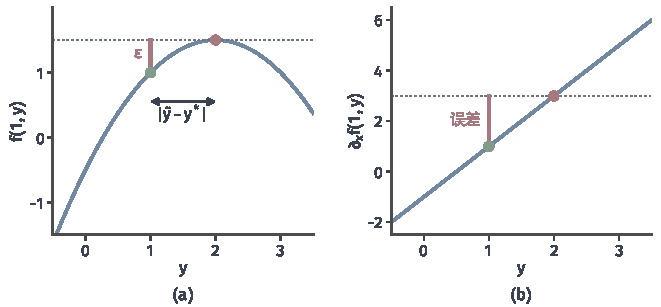
\includegraphics[width=112mm]{figures/05-optimization/07-multiple-criteria-and-nested-optimization/matplotlib/minimax-approx-response/figure.pdf}
 \caption{$f=-\frac12x^2+2xy-\frac12y^2$在$x=1$处。(a)内层函数，红点是最优响应，绿点是候选响应$\tilde{y}=1$，红线是内层间隙$\varepsilon=\frac12$，双箭头是响应距离。(b)外层偏导数关于$y$的直线，红点是真实导数$3$，绿点是候选给出的$1$，红线是误差。}
 \label{fig:minimax-approx-response}
\end{BookInlineFigure}

\paragraph{误差怎样影响外层}
梯度带误差时，外层下降还成立吗？先要知道$\phi$够光滑。下面的引理说明响应随$\bm{x}$平稳移动，从而$\phi$可微且梯度Lipschitz。这里不需要$\bm{Y}$紧。

\begin{lemma}[响应的稳定性与$\phi$的光滑性]
\label{lem:minimax-response-lipschitz}
在上述条件下，设$\bm{X}=\mathbb{R}^n$。则$\bm{y}^\star(\cdot)$是$\kappa$-Lipschitz的，$\phi$可微，梯度仍由式~\eqref{eq:minimax-danskin-gradient}的表达式给出，并且$\nabla\phi$是$L_\phi$-Lipschitz的，其中
\begin{equation}
 L_\phi=L(1+\kappa).
 \label{eq:minimax-phi-smooth}
\end{equation}
\end{lemma}

\begin{proof}
记$\bm{y}_1=\bm{y}^\star(\bm{x}_1)$，$\bm{y}_2=\bm{y}^\star(\bm{x}_2)$。两个最优性条件给出
\[
 \langle\nabla_{\bm{y}}f(\bm{x}_1,\bm{y}_1),\bm{y}_2-\bm{y}_1\rangle\leq0,\qquad\langle\nabla_{\bm{y}}f(\bm{x}_2,\bm{y}_2),\bm{y}_1-\bm{y}_2\rangle\leq0.
\]
$f(\bm{x}_2,\cdot)$的$\mu$强凹性给出
\[
 \mu\lVert\bm{y}_1-\bm{y}_2\rVert_2^2\leq\langle\nabla_{\bm{y}}f(\bm{x}_2,\bm{y}_2)-\nabla_{\bm{y}}f(\bm{x}_2,\bm{y}_1),\bm{y}_1-\bm{y}_2\rangle.
\]

右端含$\nabla_{\bm{y}}f(\bm{x}_2,\bm{y}_2)$的项由第二个最优性条件非正，可以丢掉，于是
\[
 \mu\lVert\bm{y}_1-\bm{y}_2\rVert_2^2\leq-\langle\nabla_{\bm{y}}f(\bm{x}_2,\bm{y}_1),\bm{y}_1-\bm{y}_2\rangle.
\]
在内积中加减$\nabla_{\bm{y}}f(\bm{x}_1,\bm{y}_1)$，并用第一个最优性条件丢掉一项，得到
\[
 \mu\lVert\bm{y}_1-\bm{y}_2\rVert_2^2\leq\langle\nabla_{\bm{y}}f(\bm{x}_1,\bm{y}_1)-\nabla_{\bm{y}}f(\bm{x}_2,\bm{y}_1),\bm{y}_1-\bm{y}_2\rangle.
\]
由Cauchy--Schwarz不等式和Lipschitz条件，得到
\[
 \lVert\bm{y}_1-\bm{y}_2\rVert_2\leq\kappa\lVert\bm{x}_1-\bm{x}_2\rVert_2.
\]

再证可微。任取$\bm{x}$和$\bm{d}$，记$\bm{y}=\bm{y}^\star(\bm{x})$，$\bm{y}_{\bm{d}}=\bm{y}^\star(\bm{x}+\bm{d})$，$\bm{g}=\nabla_{\bm{x}}f(\bm{x},\bm{y})$。用$\bm{y}$在$\bm{x}+\bm{d}$处的值作下界，并由光滑性，
\[
 \phi(\bm{x}+\bm{d})-\phi(\bm{x})\geq f(\bm{x}+\bm{d},\bm{y})-f(\bm{x},\bm{y})\geq\langle\bm{g},\bm{d}\rangle-\frac{L}{2}\lVert\bm{d}\rVert_2^2.
\]

用$\bm{y}_{\bm{d}}$作上界，同样由光滑性和响应的Lipschitz性，
\[
 \begin{aligned}
 \phi(\bm{x}+\bm{d})-\phi(\bm{x})&\leq f(\bm{x}+\bm{d},\bm{y}_{\bm{d}})-f(\bm{x},\bm{y}_{\bm{d}})\\
 &\leq\langle\nabla_{\bm{x}}f(\bm{x},\bm{y}_{\bm{d}}),\bm{d}\rangle+\frac{L}{2}\lVert\bm{d}\rVert_2^2\\
 &\leq\langle\bm{g},\bm{d}\rangle+L\kappa\lVert\bm{d}\rVert_2^2+\frac{L}{2}\lVert\bm{d}\rVert_2^2.
 \end{aligned}
\]
上下夹逼，得到$\phi$可微且梯度为$\bm{g}$。

最后，由梯度公式和响应的Lipschitz性，
\[
 \lVert\nabla\phi(\bm{x}_1)-\nabla\phi(\bm{x}_2)\rVert_2\leq L\lVert\bm{x}_1-\bm{x}_2\rVert_2+L\lVert\bm{y}_1-\bm{y}_2\rVert_2\leq L(1+\kappa)\lVert\bm{x}_1-\bm{x}_2\rVert_2.
\]
\end{proof}

式~\eqref{eq:minimax-phi-smooth}说明，$\phi$的光滑常数可能比$f$大$\kappa$倍。原因是响应会跟着$\bm{x}$动，$\kappa$越大响应动得越快，外层看到的函数越弯。

\begin{theorem}[带内层误差的外层下降]
\label{thm:minimax-inexact-descent}
在引理~\ref{lem:minimax-response-lipschitz}的条件下，设$\phi$有下界$\phi_{\inf}$，外层迭代$\bm{x}^{(t+1)}=\bm{x}^{(t)}-\alpha\bm{g}^{(t)}$，其中$0<\alpha\leq1/L_\phi$，$\bm{g}^{(t)}$与$\nabla\phi(\bm{x}^{(t)})$之差的范数不超过$\delta$。则
\begin{equation}
 \min_{0\leq t<T}\lVert\nabla\phi(\bm{x}^{(t)})\rVert_2^2\leq\frac{2(\phi(\bm{x}^{(0)})-\phi_{\inf})}{\alpha T}+\delta^2.
 \label{eq:minimax-inexact-descent}
\end{equation}
\end{theorem}

\begin{proof}
记$\bm{x}=\bm{x}^{(t)}$，$\bm{g}=\bm{g}^{(t)}$，$\bm{e}=\bm{g}-\nabla\phi(\bm{x})$。由$L_\phi$-光滑的下降引理和$\alpha L_\phi\leq1$，
\[
 \phi(\bm{x}^{(t+1)})\leq\phi(\bm{x})-\alpha\langle\nabla\phi(\bm{x}),\bm{g}\rangle+\frac{\alpha}{2}\lVert\bm{g}\rVert_2^2.
\]
对任意向量$\bm{a},\bm{b}$有恒等式
\[
 -\langle\bm{a},\bm{b}\rangle+\frac12\lVert\bm{b}\rVert_2^2=\frac12\lVert\bm{b}-\bm{a}\rVert_2^2-\frac12\lVert\bm{a}\rVert_2^2.
\]
取$\bm{a}=\nabla\phi(\bm{x})$，$\bm{b}=\bm{g}$，得到
\[
 \phi(\bm{x}^{(t+1)})\leq\phi(\bm{x})-\frac{\alpha}{2}\lVert\nabla\phi(\bm{x})\rVert_2^2+\frac{\alpha}{2}\lVert\bm{e}\rVert_2^2.
\]
对$t=0,\ldots,T-1$求和，用$\phi(\bm{x}^{(T)})\geq\phi_{\inf}$和$\lVert\bm{e}\rVert_2\leq\delta$，再除以$\alpha T/2$，左端的平均不小于最小值，即得结论。
\end{proof}

式~\eqref{eq:minimax-inexact-descent}有两项：第一项随$T$下降，第二项是内层误差留下的平台。要让外层梯度小到$\epsilon$，内层误差$\delta$也要到$\epsilon$量级。结合式~\eqref{eq:minimax-gradient-error}，这要求内层间隙满足$L\sqrt{2\varepsilon/\mu}\lesssim\epsilon$，即$\varepsilon$是$\mu\epsilon^2/L^2$量级。

\paragraph{计算过程}
内层用$K$步投影梯度上升，并从上一轮的响应出发，比从头开始省事，因为$\bm{x}$变化不大时响应也变化不大。仍用$f=-\frac12x^2+2xy-\frac12y^2$。

\needspace{6\baselineskip}
\paragraph{变量}
\begin{itemize}
 \item $x^{(t)}$：外层变量；
 \item $y^{(t)}$：第$t$轮内层结束后的近似响应；
 \item $K$：每轮内层步数；$\beta$：内层步长；$\alpha$：外层步长。
\end{itemize}

\paragraph{初始化}
取$x^{(0)}$和$y^{(-1)}$。例中$x^{(0)}=1$，$y^{(-1)}=0$，$K=2$，$\beta=\frac12$，$\alpha=\frac16$。内层的曲率是$1$，步长$\beta=\frac12$不超过曲率的倒数。

\needspace{6\baselineskip}
\paragraph{每轮更新}
\begin{enumerate}
 \item 从$y=y^{(t-1)}$出发做$K$次内层更新$y\leftarrow P_Y(y+\beta\partial_yf(x^{(t)},y))$，得$y^{(t)}$。例中$\partial_yf=2x-y$，第一轮
 \[
  y:\ 0\to0+\frac12\cdot2=1\to1+\frac12\cdot1=1.5,\qquad y^{(0)}=1.5.
 \]
 \item 用当前响应计算外层偏导数$g^{(t)}=\partial_xf(x^{(t)},y^{(t)})$。例中第一轮
 \[
  g^{(0)}=-1+2\cdot1.5=2.
 \]
 \item 更新外层$x^{(t+1)}=x^{(t)}-\alpha g^{(t)}$。例中第一轮
 \[
  x^{(1)}=1-\frac26=\frac23.
 \]
\end{enumerate}

第二轮内层从$y=1.5$出发，目标$2x^{(1)}=\frac43$，两步给出
\[
 y:\ 1.5\to1.41667\to1.375,\qquad y^{(1)}=1.375.
\]
外层偏导数是$g^{(1)}=-\frac23+2.75\approx2.0833$，所以$x^{(2)}\approx0.3194$。真实导数$3x^{(1)}=2$，这一轮的误差约为$0.083$。

第一轮的真实导数是$3$，误差是$1$；第二轮暖启动之后，误差降到$0.083$。迭代继续下去，到设定的外层梯度精度为止。这里用$\lvert g^{(t)}\rvert$作判据时要记住，它自身带有内层误差。

\paragraph{一般非凹内层}
上面的传递依赖强凹性。没有强凹性时，$\nabla_{\bm{y}}f$很小不说明响应接近最优。式~\eqref{eq:minimax-nonconcave}中$(x,y)=(1,-1)$的内层梯度严格为零，内层间隙却是$2.77$。此时只从$\tilde{\bm{y}}$算出的值只是$\phi(\bm{x})$的下界，真实误差不可知，外层停止时必须说明实际使用的响应证据：用了什么内层算法、多少起点、最后的残差，而不能把$\nabla_{\bm{y}}f\approx\bm{0}$说成“内层已解”。
